\title[Zahlensysteme]{Zahlensysteme und Kodierungen}

\subtitle{\emoji{woman-technologist} Texte und Farben kodieren}

\author[Blum, Cyril] % (optional)
{Cyril Blum \inst{1}}

\institute[KZN] % (optional)
{
  \inst{1}%
  Fachschaft Informatik\\
  Kantonsschule im Lee
}

\date[\today] % (optional)

\logo{
\includegraphics[width=2cm]{Logos/LeeLogo}}

\titlegraphic{\includegraphics[width=\textwidth]{"Grundlagen_Info/06_Datenbanken/Figures/title-emojis"}}

%The next statement creates the title page.
\frame{\titlepage}


\begin{frame}{Bits \& Bytes}{Übersicht}
	\begin{enumerate}
		\item \faCheckSquare{} Zählen mit Bits
		\item \faCheckSquare{} Rechnen mit Bits
		\item \faSquare{} Buchstaben codieren mit Bits
		\item \faSquare{} Farben repräsentieren mit Bits
	\end{enumerate}
\end{frame}

\begin{frame}{Buchstaben}
	\begin{center}
		Wie könnte man Buchstaben repräsentieren, wenn der Computer nur 0 / 1 kennt?
	\end{center}
\end{frame}

\begin{frame}{Buchstaben}
\gls{ASCII}
\begin{itemize}
	\item 1 Byte pro Zeichen
	\item Z.B.: \texttt{0100 0001} $\rightarrow$ A
	\item 1 Bit war reserviert zur Fehlerkontrolle
\end{itemize}
\only<2->{
\begin{center}
	\textbf{Frage}: Wie viele Zeichen kann man mit einem Byte abbilden? Wie viele Zeichen mit der \gls{ASCII}-Kodierung?
\end{center}
}
\only<3->{\[2^8 = 256,\; 2^7 = 128\]}

\only<4->{
\begin{center}
\textbf{Frage}: Was ist die grösste binäre Zahl, die man mit einem Byte abbilden kann, in hexadezimaler Zahlendarstellung?
\end{center}
}
\only<5->{\[11111111_2 = 255_{10} = FF_{16}\]}
\end{frame}

\begin{frame}[fragile]{\gls{ASCII} (Auszug)}
\begin{table}[H]
	\centering
	\tiny
	\begin{tabular}{cccc}
		\toprule
		Dezimal & Hexadezimal & Binär & Zeichen \\
		\midrule
		0 & 00 & 00000000 & NUL \\
		1 & 01 & 00000001 & SOH \\
		2 & 02 & 00000010 & STX \\
		3 & 03 & 00000011 & ETX \\
		4 & 04 & 00000100 & EOT \\\midrule
		... & ... & ... & ... \\\midrule
		36 & 24 & 00100100 & \$ \\
		37 & 25 & 00100101 & \% \\
		38 & 26 & 00100110 & \& \\
		39 & 27 & 00100111 & ' \\
		40 & 28 & 00101000 & ( \\
		41 & 29 & 00101001 & ) \\\midrule
		... & ... & ... & ... \\\midrule
		48 & 30 & 00110000 & 0 \\
		49 & 31 & 00110001 & 1 \\
		50 & 32 & 00110010 & 2 \\
		51 & 33 & 00110011 & 3 \\
		52 & 34 & 00110100 & 4 \\\midrule
		... & ... & ... & ... \\\midrule
		65 & 41 & 01000001 & A \\
		66 & 42 & 01000010 & B \\
		67 & 43 & 01000011 & C \\
		68 & 44 & 01000100 & D \\
		69 & 45 & 01000101 & E \\\midrule
		... & ... & ... & ... \\\bottomrule
	\end{tabular}
\end{table}
\end{frame}

\begin{frame}[fragile]{\emoji{keyboard} \gls{ASCII}}
	\begin{center}
		Jedes Zeichen der damaligen Tastatur kodiert
	\end{center}
\end{frame}

\begin{frame}[fragile]{\gls{UTF-8}}
\begin{figure}
\centering
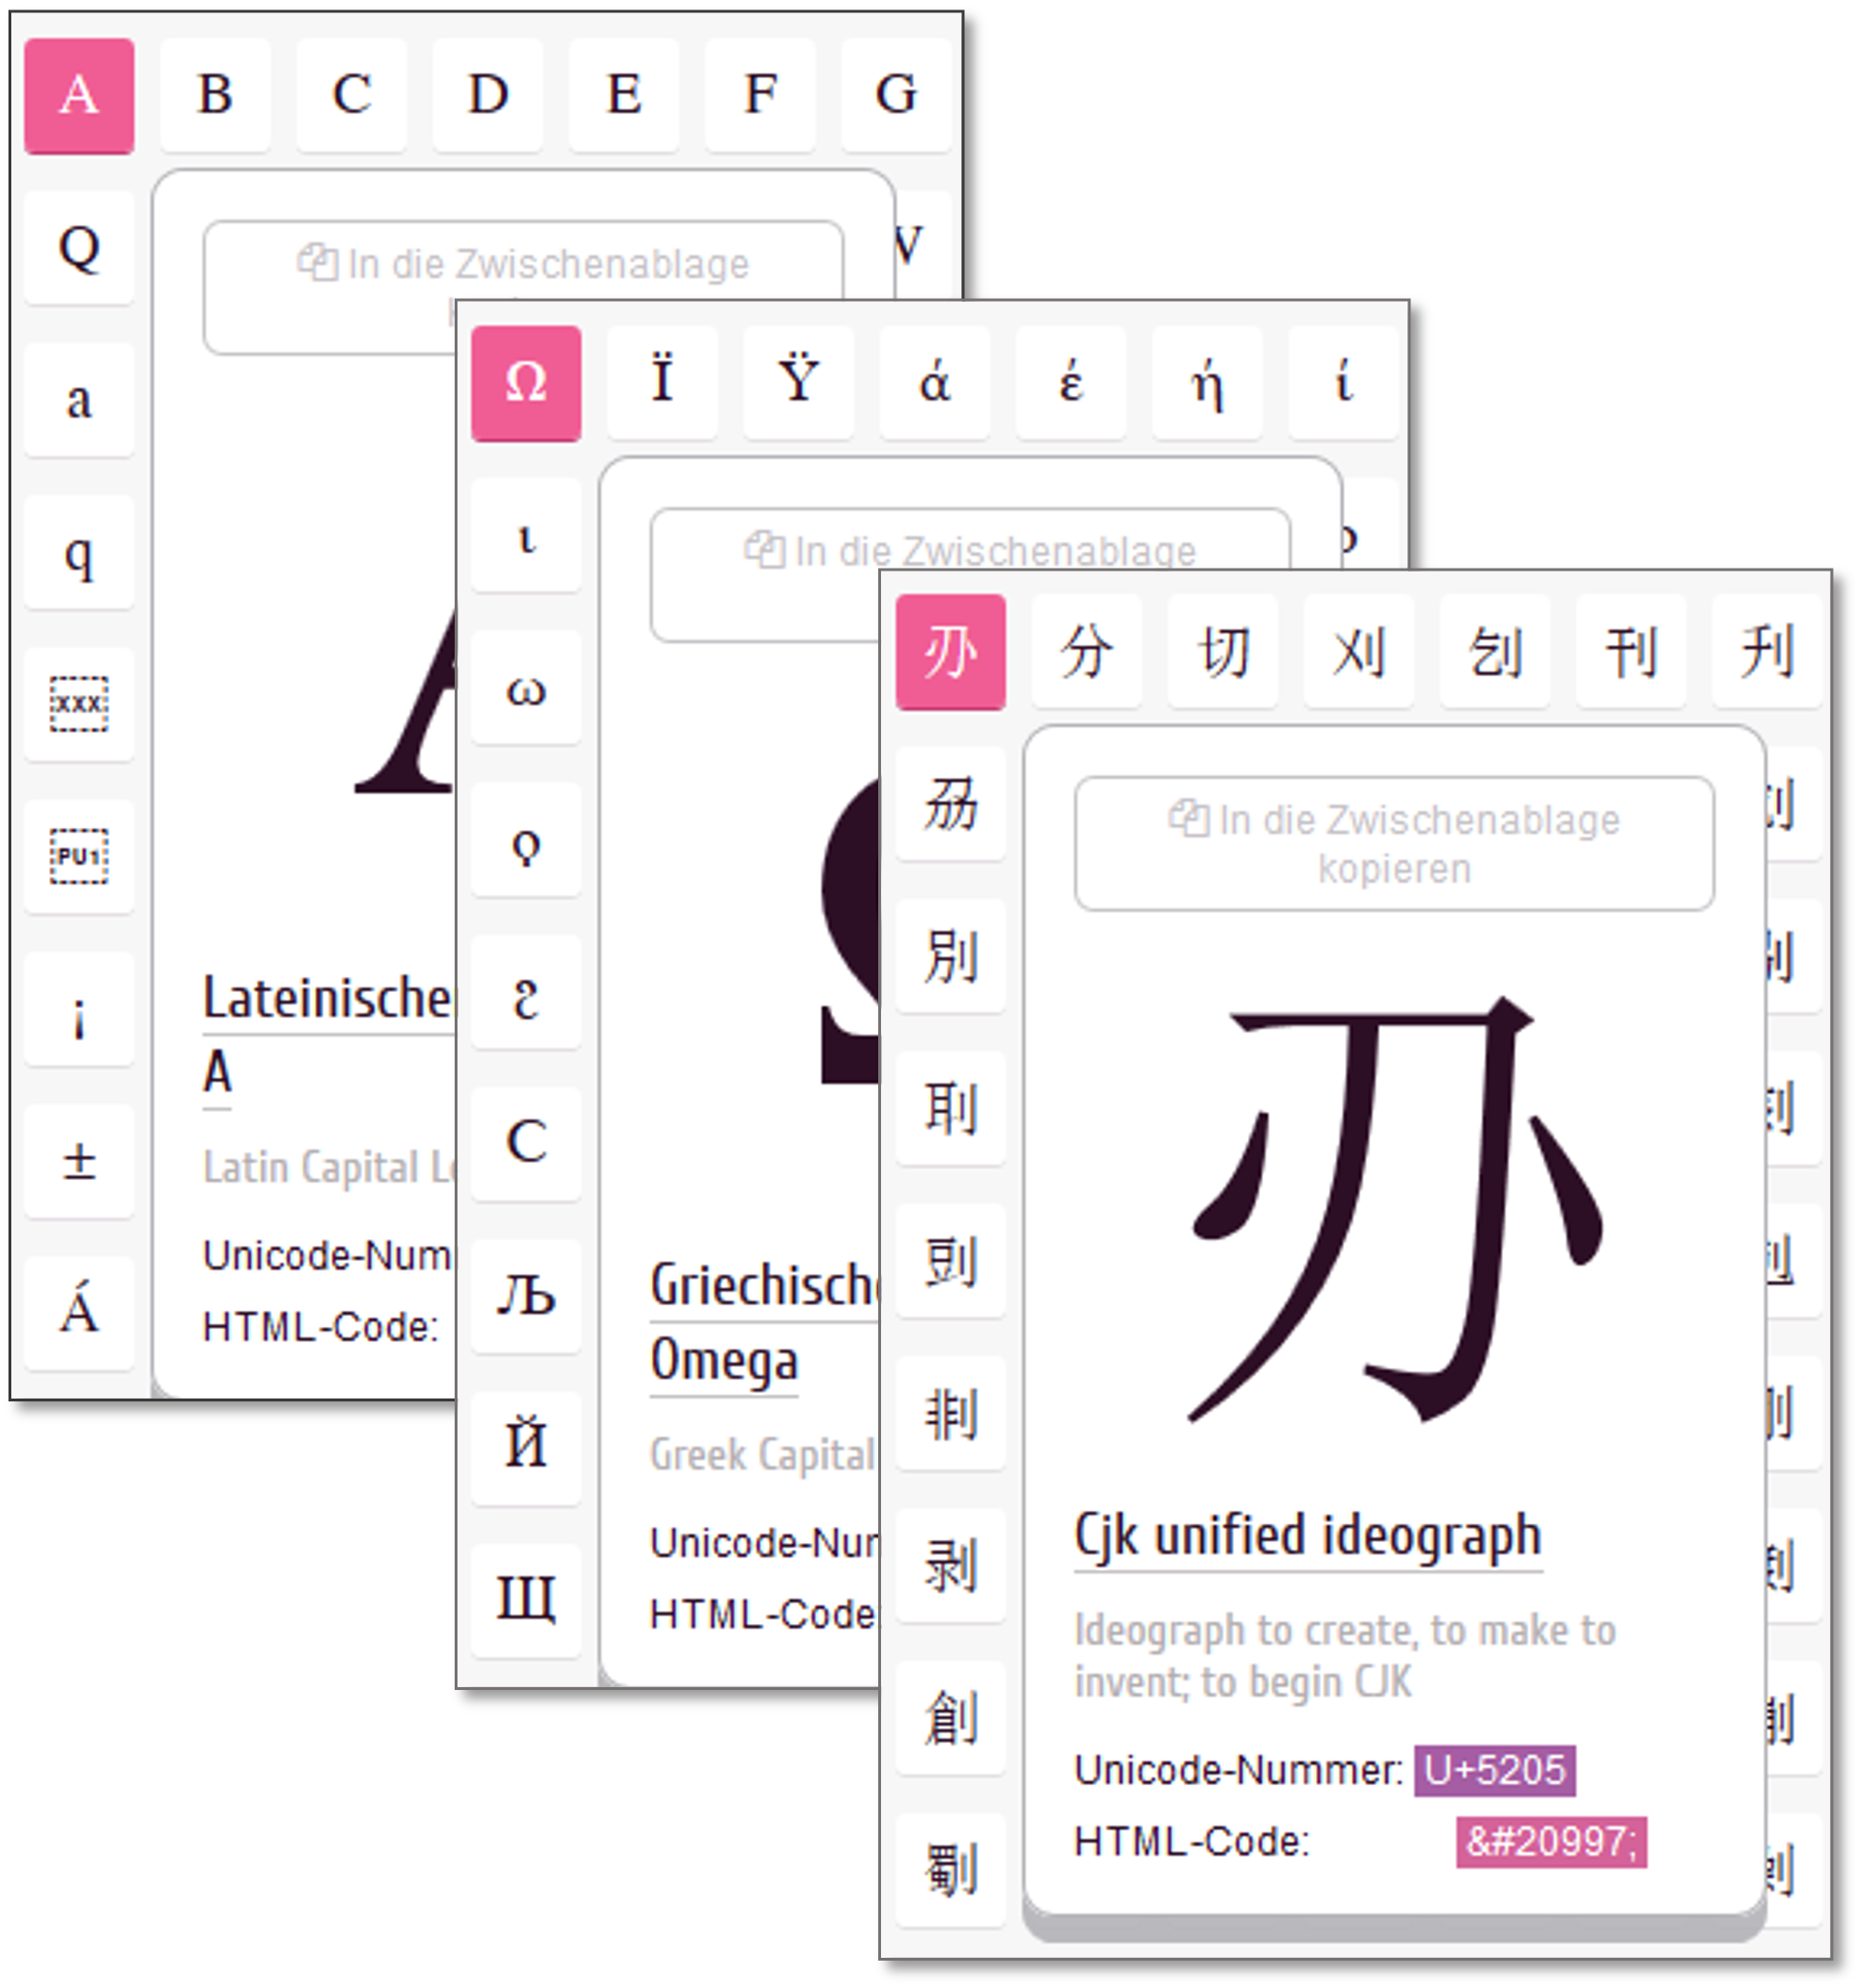
\includegraphics[width=0.5\linewidth]{Grundlagen_Info/01_TheoretischeInformatik/Figures/UTF8}
\end{figure}
\begin{center}
1-4 Bytes für jedes Zeichen zur Verfügung, allerdings nur ein Teil davon nutzbar.
\end{center}
\end{frame}


\begin{frame}[fragile]{Farben kodieren}
	\begin{table}[H]
		\centering
		\begin{tabular}{lllll}
			1 & 0 & 0 & 0 & 1 \\
			0 & 1 & 0 & 1 & 0 \\
			0 & 0 & 1 & 0 & 0 \\
			0 & 1 & 0 & 1 & 0 \\
			1 & 0 & 0 & 0 & 1
		\end{tabular}
	\end{table}
	\begin{center}
		Welches Bild wird dargestellt?\\
		Wie viele Bit Speicherplatz benötigt das Bild?
	\end{center}
\end{frame}

\begin{frame}[fragile]{Farben kodieren}{\glspl{LED} in Bildschirmen}
	\begin{figure}[H]
		\centering
		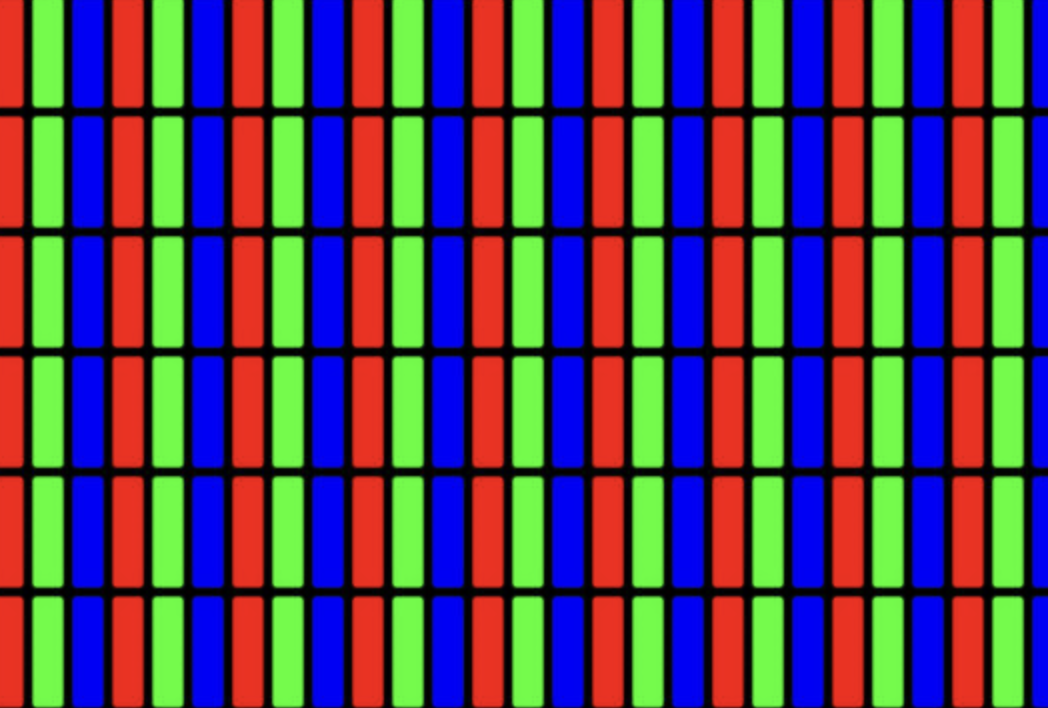
\includegraphics[width=0.5\linewidth]{Grundlagen_Info/01_TheoretischeInformatik/Figures/pixels}
	\end{figure}
\end{frame}

\begin{frame}[fragile]{Farben kodieren}
	\begin{figure}[H]
		\centering
		\begin{subfigure}{.49\textwidth}
			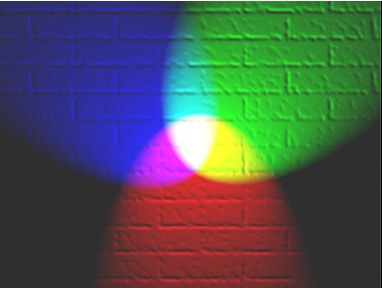
\includegraphics[width=\textwidth]{Grundlagen_Info/01_TheoretischeInformatik/Figures/rgb-farbmischung-1}
		\end{subfigure}
		\begin{subfigure}{.49\textwidth}
			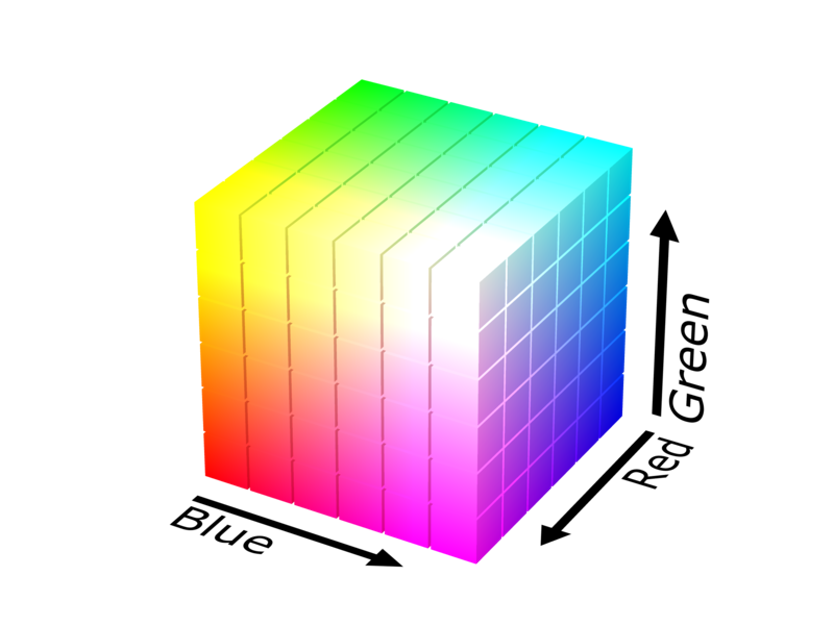
\includegraphics[width=\textwidth]{Grundlagen_Info/01_TheoretischeInformatik/Figures/rgb-farbmischung-2}
		\end{subfigure}
	\end{figure}
	$\rightarrow$ Jede Farbe kodiert zwischen 0 und 255!
	\only<2->{
	\red{11111111}\green{00000000}\blue{00000000} = \#\red{FF}\green{00}\blue{00} = \red{255}, \green{0}, \blue{0} = reines Rot\\
	
	\red{10000000}\green{10000000}\blue{10000000} = \#\red{80}\green{80}\blue{80} = \red{128}, \green{128}, \blue{128} = grau}	
\end{frame}

\begin{frame}{Farben}{Farbtiefe}
	\begin{figure}[H]
		\centering
		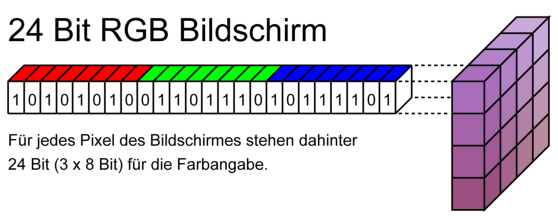
\includegraphics[width=\linewidth]{Grundlagen_Info/01_TheoretischeInformatik/Figures/colordepth}
	\end{figure}
\end{frame}

\begin{frame}{Farben}{Farbtiefe}
	\begin{figure}[H]
		\centering
		\begin{subfigure}{.49\textwidth}
			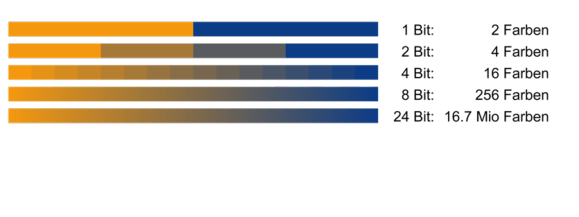
\includegraphics[width=\textwidth]{Grundlagen_Info/01_TheoretischeInformatik/Figures/colordepth-bar}
			\caption{Farbtiefe: Skala}
			\label{fig:colordepth-bar}
		\end{subfigure}
		\begin{subfigure}{.49\textwidth}
			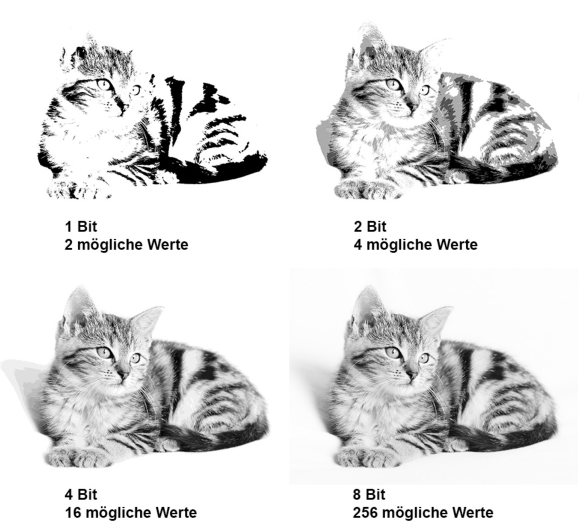
\includegraphics[width=\textwidth]{Grundlagen_Info/01_TheoretischeInformatik/Figures/colordepth-cat}
			\caption{Farbtiefen bei Schwarz-Weiss-Bildern}
			\label{fig:colordepth-cat}
		\end{subfigure}
		\caption*{Farbtiefe: Beispiele}
		\label{fig:colordepth-examples}
	\end{figure}
\end{frame}

\begin{frame}{Speichergrössen}
	\begin{table}[H]
		\footnotesize
		\centering
		\begin{tabular}{@{}l|rr|l@{}}
			\toprule
			\textbf{Masseinheit} & \multicolumn{2}{l|}{\textbf{Dezimalsystem}} & Grössenordnung                                   \\ \midrule
			KB (Kilobyte)        & $10^3$ B(yte)                               & 1'000 B             & eine Text-Datei            \\
			MB (Megabyte)        & $10^6$ B                                    & 1'000'000 B         & eine Musik-Datei           \\
			GB (Gigabyte)        & $10^9$ B                                    & 1'000'000'000 B     & eine Video-Datei           \\
			TB (Terabyte)        & $10^{12}$ B                                 & 1'000'000'000'000 B & kleiner Firmen-Server      \\
			PB (Petabyte)        & $10^{15}$ B                                 & ...                 & Facebook-Server            \\
			EB (Exabyte)         & $10^{18}$ B                                 & ...                 & alle CERN-Daten            \\
			ZB (Zettabyte)       & $10^{21}$ B                                 & ...                 & alle Daten ($\sim$ 100 ZB) \\
			YB (Yottabyte)       & $10^{24}$ B                                 & ...                 & $\sim$ 2030?               \\ \bottomrule
		\end{tabular}
		\caption*{Gängige Daten-Grössenordnungen in der Informatik}
	\end{table}
	\only<2->{
	\begin{center}
		Wie nennt man ein \enquote{Megagramm} geläufiger?
		\end{center}}
\end{frame}

\begin{frame}[fragile]{Auftrag}{Skript auf Moodle}
	\begin{itemize}
		\item Buchstaben: \acrshort{ASCII} und \acrshort{UTF-8}
		\begin{itemize}
			\item \aufgabebox{Aufgaben 2.3-2.7}
		\end{itemize}
		\item Bilder
		\begin{itemize}
			\item \aufgabebox{Aufgaben 2.8-2.16 (\emoji{trophy} 2.13)} 
		\end{itemize}
		\item \challengebox{Kurs auf Moodle (mit Tests)}
	\end{itemize}
\end{frame}